% GraphAudit, SIGMOD 2027 demonstration track. First full draft, 2026-11-25.
% Call (read 2026-11-25): 4 US-letter pages INCLUDING bibliography, \documentclass[sigconf,9pt]{acmart},
% margins and spacing unchanged, not double-blind (authors and affiliations must appear).
% Every number is traced in NOTES.md.
\documentclass[sigconf,9pt]{acmart}

\settopmatter{printacmref=false}
\setcopyright{none}
\renewcommand\footnotetextcopyrightpermission[1]{}
\acmConference[SIGMOD '27]{ACM SIGMOD International Conference on Management of Data}{June 13--18, 2027}{Huntington Beach, CA, USA}
\emergencystretch=1em

\usepackage{booktabs}

\newcommand{\sys}{GraphAudit}

\begin{document}

\title{GraphAudit: Verifiable Conversational Graph Analytics with Computation Reuse}

% Sole author (confirmed 2026-11-26). The call asks for a CMT account and an ORCID.
% TODO: add the e-mail address and the ORCID by hand before submission; both are left out of the draft on purpose.
\author{Xiaofei Zhang}
\affiliation{%
  \institution{University of Memphis}
  \city{Memphis}
  \state{Tennessee}
  \country{USA}}

\begin{abstract}
Analysts ask a graph a sequence of related questions, and a language-model assistant that keeps state
between them can answer a follow-up from a result that is no longer valid: the data file has grown, or the
follow-up reads the graph differently. We demonstrate \sys{}, which turns each question into a typed plan
over a catalogue of 76 checked operators and stores every step result under a key that covers the file
contents, the reading of the graph, the parameters and all inputs. A result is reused only when its key
matches. A request with two readings is shown as two contracts and nothing runs until one is chosen; a
request outside the catalogue is answered by two independently written functions that must agree, or is
declined. Attendees drive a seven-step session on the Pokec social network (30.6 million links), change
the data file themselves, and compare each turn with a code-writing agent that keeps its variables.
Video: \emph{[URL to be added]}.
\end{abstract}

\keywords{graph analytics, natural-language interfaces, computation reuse, verification, LLM agents}

\maketitle

\section{Introduction}

A language model can turn ``who are the ten most influential users?'' into code that loads an edge file and
runs PageRank. Real analysis is a session: \emph{which regions are they from}, \emph{show the top 20
instead}, \emph{and within this region?} Systems for such sessions keep state. A notebook-style agent keeps
Python variables between turns~\cite{codeact}, which makes follow-ups cheap, and which is where a session can
go wrong without any sign of it.

\textbf{The data changes underneath.} A nightly load appends rows to the edge file and the analyst asks the
next question. An agent that kept the graph in memory answers from the old graph. We measured this
(Section~\ref{sec:evidence}): an agent with a persistent Python process gave stale answers in every run we
made, with a small and with a large model. Telling it that the file may change removed the stale answers
with the large model, at the price of recomputation, and did not on large graphs with the small one.

\textbf{The reading changes underneath.} ``Most influential within region $X$'' can mean the whole-graph
scores listed for the members of $X$, or scores recomputed on the subgraph induced by $X$. The first reuses
the earlier result and the second must not. Over 60 group restrictions on real profile data the two
readings gave a different top-10 set in all 60 and shared 3.7 of 10 nodes on average. An assistant that
picks one in silence returns a well-formed answer to a question the analyst may not have asked.

\textbf{Approach.} Generated code runs, but it is not an analysis whose semantics, assumptions and reuse can
be examined. \sys{} places an explicit contract between the question and the computation: a typed plan over
a fixed operator catalogue, executed by an engine that owns loading, the reading of the file and the result
store. Reuse then becomes a property of keys, not a judgment of the model. We do not claim that typed plans
are more accurate than generated code; in a pilot on sessions that contain no trap the two did not separate on accuracy. The
claim is narrower: wrong reuse is excluded by construction, and what was assumed, reused and not checked is
on screen.

\textbf{Contributions.} (1) A session engine with lineage-keyed reuse that detects file changes and reading
changes without being told. (2) A two-contract clarification for scope-ambiguous requests, produced by a
mechanical plan rewrite. (3) Plan replay for repeated questions and a checked code fallback for requests
outside the catalogue, with declined requests and loading conventions stated instead of hidden. (4) A
demonstration in which the audience changes the data and watches both \sys{} and a stateful code agent
respond.

\begin{figure}[t]
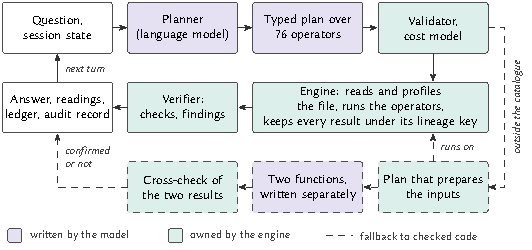
\includegraphics[width=\linewidth]{figs/fig1-architecture.pdf}
\caption{Architecture of \sys{}. The model writes plans and, in the fallback, two functions; loading, the
reading of the file, the result store and every check belong to the engine.}
\label{fig:arch}
\end{figure}

\section{System}
\label{sec:system}

\sys{} (Figure~\ref{fig:arch}) is written in Python on igraph~\cite{igraph}. It reads an edge file with an
optional node table, and has been run on files of up to 117 million links.

\textbf{Profile and typed plans.} On load, the engine derives file facts and a profile card: size, inferred
direction and weights with the evidence for each, node attributes with type and coverage. The planner model
sees the card, the catalogue and a compact session record, and returns a plan: a list of steps, each an
operator from the catalogue with typed arguments that may refer to earlier steps, together with the
interpretation it assumed. The 76 operators cover counts, degrees and centralities, components and cores,
communities, paths, attribute filters and groupings, arithmetic on results, and graph-reading operators
such as the undirected or the mutual-link graph. A validator checks operators, types, references, attribute
names and category values; a cost model rejects a plan over budget before anything runs; a verifier
attaches findings to the answer (for example, that PageRank scores sum to one).

\textbf{Lineage-keyed result store.} Every step result is stored under
\[
k(s)=H\bigl(\mathit{op},\ \mathit{params},\ \mathit{reading},\ \mathit{seed},\
k(\mathit{in}_1),\dots,k(\mathit{in}_n)\bigr),
\]
with parameters in canonical form (defaults written out), whose root is a hash of the whole edge file and node table together with the reading under which the graph
was loaded. PageRank on an induced subgraph cannot collide with PageRank on the whole graph, and a changed
reading or file changes every key downstream. Rankings are always cut from stored full score maps, so ``top
20 instead'' is an exact reuse and never an extension of a list of ten. Before each turn the engine compares
the file's size and modification time and, if they moved, its hash. On a change it reloads the graph, or
appends in place when the file only grew and a set of conditions guarantees the same graph as a full load,
and reports \texttt{data\_changed} in the turn.

\textbf{Session state and two contracts.} The planner never sees the chat history or raw values. It sees
the accepted reading, earlier plans with result sizes, the current selection that ``them'' refers to, and
standing settings (``use damping 0.9 from now on''). It returns a complete plan that copies earlier steps
unchanged; the engine recognises them by key, so each turn's outcome is derived, not declared: exact reuse,
partial reuse, recompute, or clarify. Operators are marked scope-sensitive. When a plan restricts a
scope-sensitive measure to a group, the engine rewrites the plan into its other reading and returns both as
contracts (compute on the whole graph, then list the group; or compute on the group's subgraph), each with
what it would reuse. Nothing executes until the user chooses, and the choice is carried to later turns and
stated there.

\textbf{Replay and prompt caching.} A question repeated word for word runs its earlier plan with no planner
call, but only if that plan was self-contained (no reference to an earlier turn, no setting, no open
reading) and the settings in force are unchanged. The plan is still validated and executed against the
data as it then is, so replay removes the planner call and never a check. The catalogue, the rules and the
profile card are sent as a cached prompt prefix.

\textbf{Checked code fallback, declined requests, conventions.} When no combination of operators computes
exactly what is asked, the planner must say so and name the missing capability; it may not answer an easier
question. With the fallback on, a second plan prepares the inputs with catalogue steps (select the nodes,
induce the subgraph, drop direction) and states the task. Two functions are then written by two model calls
that do not see each other, one told to prefer igraph's routine and the other to avoid it, and each runs in
its own process on the prepared inputs. Neither reads the file. If both return the same value the turn is
an \emph{answer by code}, shown as a lower grade of answer than an operator answer; otherwise it is
\emph{not confirmed}, and both candidates are shown without an answer. Both writers read one task statement,
so a wrong reading of the question passes this check; we return to this in Section~\ref{sec:evidence}.
Finally, loading conventions that change counts are printed with every answer: on LiveJournal, 518,382 of
the 68,993,773 rows link a node to itself and are left out of the graph, and each answer says so.

\begin{figure*}[t]
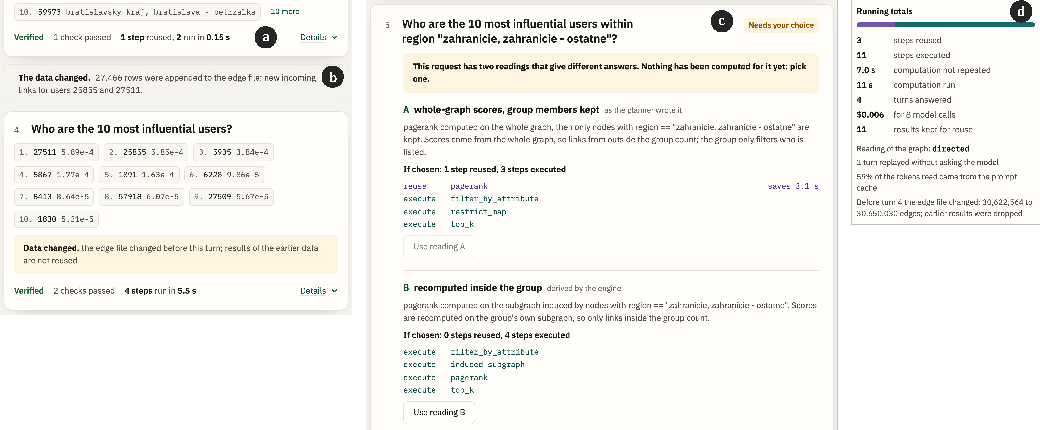
\includegraphics[width=\textwidth]{figs/fig2-session.pdf}
\caption{The session page at the scope-ambiguity step of the signature session on Pokec: (a) steps reused
by lineage key, (b) the file change noticed without being announced, (c) two contracts, with nothing
executed until one is chosen, (d) the ledger of reused and executed steps, model calls and replayed turns.}
\label{fig:session}
\end{figure*}

\section{Demonstration}
\label{sec:demo}

The demonstration uses the Pokec social network from SNAP~\cite{snap} with its profile table: 1,632,803
users, 30,622,564 directed friendship links, and attributes such as region, age and gender. It has three parts.

\textbf{The signature session.} Seven steps, scripted as data and playable live or from a recording
(Figure~\ref{fig:session}).
\emph{(1)} ``Who are the 10 most influential users?'' The plan, the reading of the file and the measure
chosen for ``influential'' (PageRank) are shown with the answer.
\emph{(2)} ``Which region is each of them from?'' Two steps are marked reused; one attribute lookup runs.
\emph{(3)} ``Show the top 20 instead.'' Only the final cut runs; the scores are reused.
\emph{(4)} The edge file grows by 27,466 rows. Nobody tells the system.
\emph{(5)} The words of step 1 again. The plan is replayed with no planner call, the turn reports
\texttt{data\_changed}, nothing computed on the old file is reused, and two users who gained links now lead
the ranking.
\emph{(6)} The same question ``within region $X$'': two contracts appear and nothing runs. Reading B is
chosen and then A is shown beside it; the two top-10 lists share 4 users.
\emph{(7)} ``Among the 20 most influential users, what is the largest group in which every two are
friends?'' The catalogue has no maximum-clique operator and says so; four checked steps prepare the 20-user
subgraph, two functions agree on a group of 5, and the answer is marked as an answer by code, with the task
statement and both functions one click away.
The ledger closes the session: in the recording, 6 steps reused and 20 executed, 1 turn replayed, 15 model
calls for about one cent on Claude Haiku 5.5, and 61\% of input tokens read from the prompt cache. The
audit record holds every plan, every reuse decision with its key, and every finding.

\textbf{The live path.} Against a server holding the graph, visitors type their own questions or pick the
script's. A button labelled ``Change the data file'' appends rows on disk and tells the session nothing;
the next question shows whether the change was noticed. In our check of this path all seven steps gave the
recorded outcomes; a session starts in about 35 seconds (copying and loading Pokec) and turns take 5 to 30
seconds, most of it the model. If the network fails, the recorded session replays in the browser with no
server and no model.

\begin{figure}[t]
\centering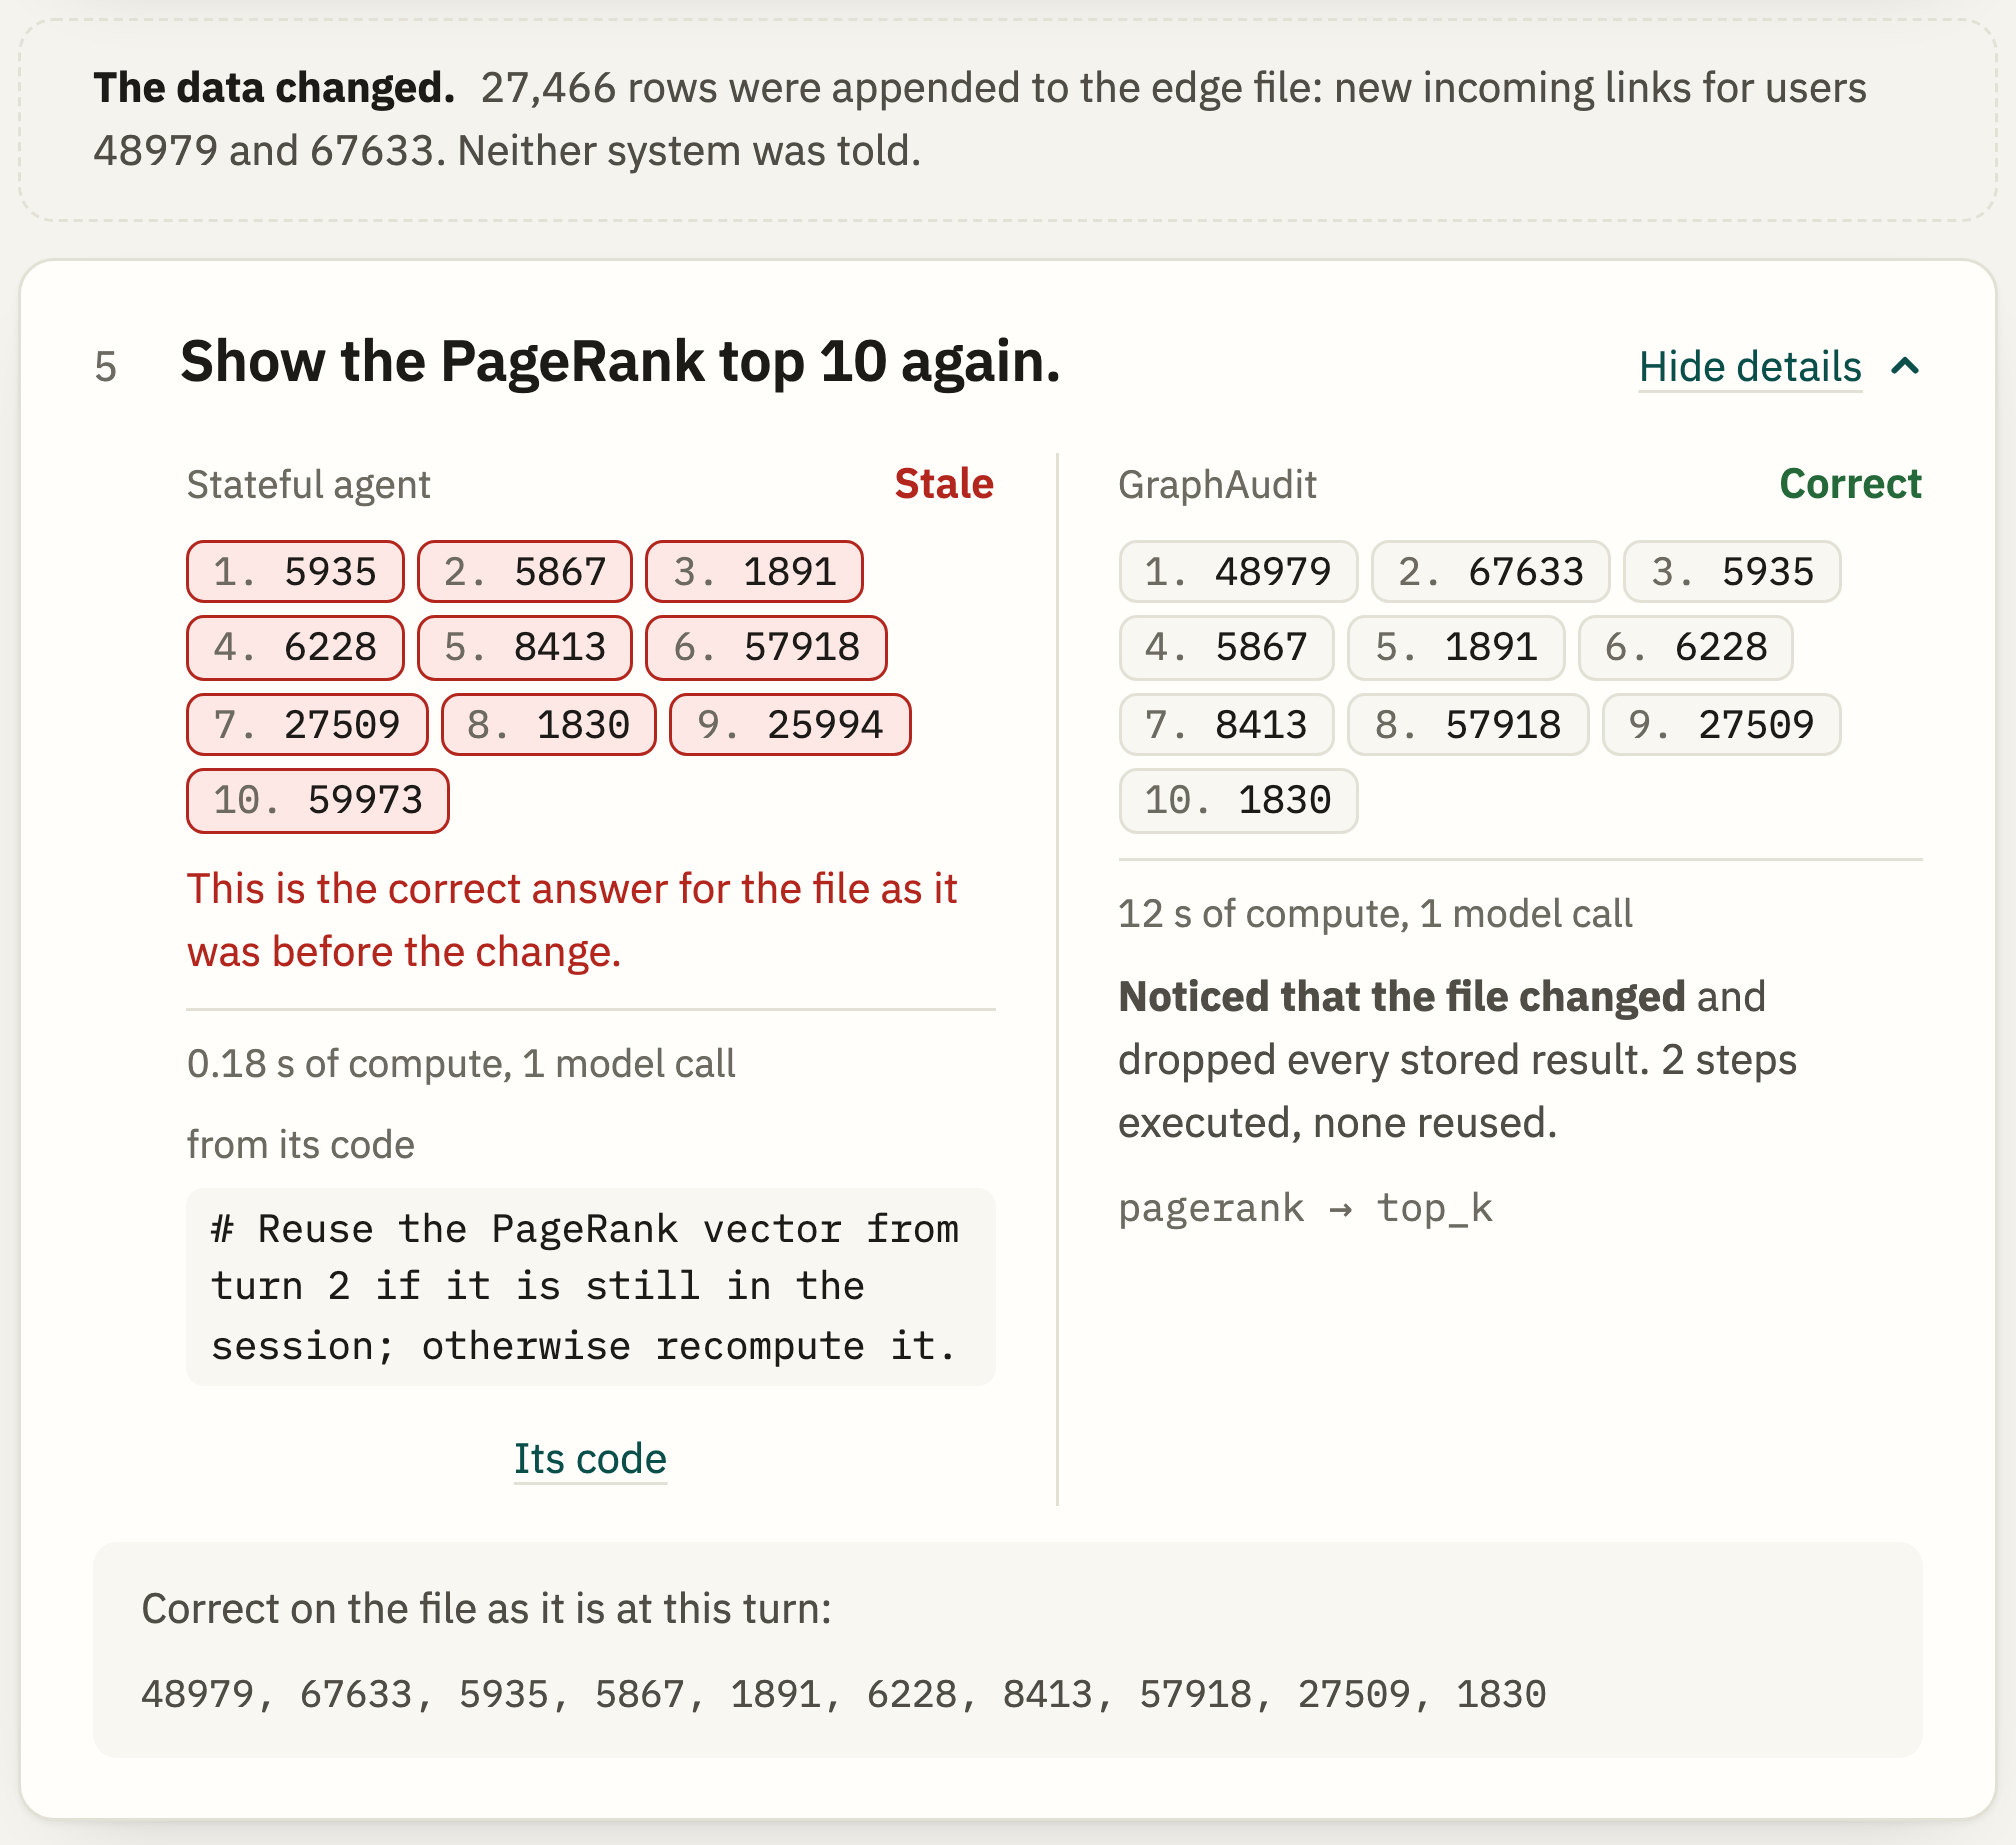
\includegraphics[width=0.68\linewidth]{figs/fig3-compare.png}
\caption{Side by side on the refresh session: after the file grows, the stateful agent reuses its PageRank
vector (the deciding line of its code is quoted) while \sys{} reports the change and recomputes.}
\label{fig:compare}
\end{figure}

\textbf{Side by side with a stateful code agent.} The third page (Figure~\ref{fig:compare}) replays one
stored run of each system on a ten-question ``morning dashboard'' session on Pokec during which the same
27,466 links are appended. Each row shows both answers with the harness's verdict (correct, stale, wrong),
compute time and model calls; for the agent it quotes the line of its own code that decides the reuse. In
this run, on Haiku, the agent is correct on 5 of 10 turns, stale on 3 and wrong on 2 more after the change; \sys{} is correct on 10 of 10. The agent used 19 seconds of compute and \sys{} 48, of which 29
are loading; model fees are \$0.006 and \$0.005. The page states that this is one run and that the agent's
result depends on the model and on a warning: on this session the warned agent on Claude Opus 5.5 was right
on every turn in three runs.

\textbf{What attendees do.} They ask Pokec their own questions; press the data-change button when they choose; pick a reading at a
two-contract card and open the other to see how far the lists differ; ask for something outside the
catalogue (a maximum clique, a matching, a maximum flow) to see a declined request, an answer by code or
a withheld answer; open the audit record; and upload their own edge list to see how its direction and
weights are inferred.

\section{Evidence}
\label{sec:evidence}

Runs used Claude Haiku 5.5 and Opus 5.5. Baselines: three code
agents of ours, given the same file facts (\emph{stateful}: one Python process per session;
\emph{warned}: told that the file may change; \emph{independent}: a fresh script per
turn), and two others: the LangGraph CodeAct agent~\cite{codeact}, plain and warned, and
GraphTeam~\cite{graphteam} with its published prompts and knowledge base; we supplied the model
client, the sandbox (a script, no container) and the search embeddings (an open model), and gave
each turn the earlier questions and its answers.

\textbf{Key ingredients.} In 246 templated fault scenarios and 201 valid-reuse scenarios on nine graphs,
with no model, the full key served no wrong value and reused all 390 valid steps; removing any one
ingredient admitted 12 (node table) to 117 (input lineage) wrong values. These are fault classes
covered, not rates in real use.

\begin{table*}[t]
\caption{Sessions with reuse traps. Correct turns [stale answers] are ranges over runs; the rest are
means: \emph{time} in seconds outside the model, with loading; \emph{tokens} in millions, in and out;
model \emph{fees} in cents (Haiku) or dollars (Opus). E2b: 22 sessions on three Pokec regions and two small
graphs. E4: 8-turn sessions on Pokec, LiveJournal and Orkut. P: four sessions on Pokec, with prompt
caching (\sys{} and our agents only) and plan replay. Traps: 47, 6, 6. Runs: 3 to 6; CodeAct on Opus 1.}
\label{tab:traps}
\footnotesize
\renewcommand{\arraystretch}{0.88}
\setlength{\tabcolsep}{5pt}
\begin{tabular}{@{}ll crrr crrr crrr@{}}
\toprule
 & & \multicolumn{4}{c}{E2b (122 turns)} & \multicolumn{4}{c}{E4 (24 turns)} & \multicolumn{4}{c}{P (43 turns)} \\
\cmidrule(lr){3-6}\cmidrule(lr){7-10}\cmidrule(l){11-14}
Model & System & Correct & Time & Tokens & Fees & Correct & Time & Tokens & Fees & Correct & Time & Tokens & Fees \\
\midrule
Haiku & \sys{}            & 122 [0]         & 331  & 1.16 & 15.6 & 24 [0]        & 257  & 0.22 & 2.9 & 42 [0]        & 188 & 0.33 & 2.0 \\
 & Stateful agent    & 107--118 [2--6] & 388  & 0.59 & 10.8 & 13 [5--6]     & 332  & 0.15 & 2.5 & 29--30 [5--6] & 147 & 0.31 & 2.6 \\
 & Warned agent      & 114--120 [0--1] & 366  & 0.63 & 11.6 & 12--15 [5--6] & 459  & 0.18 & 3.2 & 33--40 [2--5] & 361 & 0.36 & 3.2 \\
 & Independent agent & 111--122 [0]    & 407  & 0.62 & 11.7 & 23--24 [0]    & 1318 & 0.17 & 3.1 & 43 [0]        & 659 & 0.36 & 3.3 \\
 & CodeAct           & 103--114 [1--4] & 386  & 1.14 & 16.2 & 13--14 [6]    & 381  & 0.23 & 3.1 & 30--33 [5--6] & 247 & 0.37 & 4.6 \\
 & CodeAct, warned   & 111--117 [0--2] & 429  & 1.34 & 19.2 & 15--20 [2--6] & 504  & 0.30 & 4.1 & 41--42 [1]    & 741 & 0.61 & 7.7 \\
 & GraphTeam         & 81--85 [0--2]   & 1091 & 1.40 & 37.2 & --            & --   & --   & --  & --            & --  & --   & --  \\
\midrule
Opus & \sys{}            & 122 [0]         & 324  & 1.14 & 5.86 & 24 [0]        & 239  & 0.22 & 1.10 & 43 [0]       & 183 & 0.40 & 0.67 \\
 & Stateful agent    & 114--117 [5--6] & 191  & 0.40 & 2.33 & 13 [6]        & 396  & 0.11 & 0.59 & 33--41 [2--5] & 156 & 0.23 & 0.51 \\
 & Warned agent      & 121--122 [0]    & 295  & 0.49 & 3.10 & 24 [0]        & 741  & 0.14 & 0.88 & 43 [0]       & 355 & 0.30 & 0.85 \\
 & Independent agent & 121--122 [0]    & 677  & 0.53 & 3.43 & 24 [0]        & 1720 & 0.17 & 1.08 & 43 [0]       & 958 & 0.34 & 0.97 \\
 & CodeAct           & 108 [5]         & 174  & 0.99 & 5.84 & --            & --   & --   & --   & --           & --  & --   & --   \\
 & CodeAct, warned   & 109 [0]         & 259  & 1.09 & 5.87 & --            & --   & --   & --   & --           & --  & --   & --   \\
\bottomrule
\end{tabular}
\end{table*}

\textbf{Sessions with reuse traps.} Table~\ref{tab:traps} compares the systems on three sets of sessions
with reuse traps.
\emph{Accuracy.} \sys{} is never stale, and it alone is correct on every turn of E2b and E4 in every run
(in P, Haiku misreads one ``them'' in each run). Agents that keep their variables are stale in every run
with both models, and the framework agent behaves like ours. A warning removes this with Opus only. So
agents can avoid stale answers, with the large model and a warning or by recomputing everything; \sys{}
does so by construction, with the small model.
\emph{Time.} Most of \sys{}'s time is one load and profile per session. On the large graphs it needs a
third of the warned Opus agent's time and a fifth to a seventh of the independent agent's. On the small
graphs of E2b loading dominates, and most Opus agents finish sooner.
\emph{Tokens and fees.} \sys{} sends its operator catalogue with every question, so without caching it
reads up to twice the tokens of our agents and costs more on E2b: as much as CodeAct, under half
of GraphTeam. With caching on both sides (P) fees are about equal (Opus: \$0.80 without plan replay), and
we claim no advantage.
\emph{GraphTeam} keeps nothing and is rarely stale. Its errors are mostly rankings on the Pokec regions: it usually
calls NetworkX PageRank, whose default stopping rule is loose at this size (12 of 91 turns correct; 46 of
48 with igraph): a library default, not a session effect.

\textbf{Coverage on questions we did not write.} Two writer models (Opus 5.5, Qwen3-14B), told nothing about
the system, wrote 429 conversational questions on three graphs; we restated the task types of
GraphArena~\cite{grapharena}, NLGraph~\cite{nlgraph} and the benchmarks GraphTeam is evaluated on as 101
stand-alone questions. Over three runs on Haiku, \sys{} answered 399--406 and 95--100. An Opus judge
found 316--317 and 87--93 answers the same as an independent Opus script agent's; another 39--42
written answers equal a variant that script itself prints (such as ``self-loops excluded''), which leaves
33--43 and 2--4 different. Before an operator fix and the fallback, \sys{} answered 63 of the published
questions and declined the rest, among them all six NP-complete GraphArena tasks. The
reference is itself a model, so ``different'' is disagreement, not error; one reader labelled the 60
questions that differ in all three runs. 40 follow a convention or reading the reference lists, 11 turn on
an open choice or a randomised algorithm, \sys{} is wrong in 8 and the reference in 1. No check flagged the
8 errors; three share one cause, a misread ``them''.

\textbf{Errors that passed every check.} Reading results by hand found errors no check caught. On a
directed graph, a plan for ``ignoring direction'' counted a pair linked both ways twice. Of 47 confirmed
code answers, 2 were wrong because the shared task statement changed the question; that statement is the
weak point of the fallback. No rule covers what ``again'' refers to.

\section{Related Work}

Benchmarks for language models on graph problems, such as NLGraph~\cite{nlgraph} and
GraphArena~\cite{grapharena}, place a small graph in the prompt and pose single questions. Agent systems
such as GraphTeam~\cite{graphteam} and CodeAct~\cite{codeact} have the model write and run code, and
CodeAct-style agents keep variables across turns: reuse without a validity condition, which is the baseline
of our comparison. GraphSeek~\cite{graphseek} is the closest system in design; it also separates planning by the model, over a catalogue of operations, from deterministic execution,
on a graph database. \sys{} works on
files and adds the session layer: reuse decided by keys, change detection, and clarification of scope.
Conversational text-to-SQL (SParC~\cite{sparc}, CoSQL~\cite{cosql}) translates every turn over a fixed
database and does not ask when an earlier result may stand in for a new computation. Helix~\cite{helix} reuses intermediate results across iterations of a machine-learning workflow, or
recomputes them when that is cheaper; the workflow there is a program, not a conversation.

\section{Status}

\textbf{Implemented and shown:} everything in Sections~\ref{sec:system} and~\ref{sec:demo},
including the live session, the data-change button, the fallback and the side-by-side page. \textbf{Planned before the conference:} recordings of further sessions; a second reader for the hand labels, and labels for the answers
that differ in only some runs; a check on the referent of ``them''; showing the task statement of a code answer to the user as the contract of the turn; and
GraphTeam on the large model.

\bibliographystyle{ACM-Reference-Format}
\bibliography{refs}

\end{document}
